\documentclass[11pt,aspectratio=169]{beamer}

\usetheme{Singapore}
\usecolortheme{orchid}

\usepackage[utf8]{inputenc}
\usepackage[russian]{babel}
\usepackage{amsmath}
\usepackage{amsfonts}
\usepackage{amssymb}
\usepackage{graphicx}
\usepackage{bibentry}
\usepackage{wasysym}
\usepackage[most]{tcolorbox}
\usepackage[normalem]{ulem}

\usepackage{hyperref}

\definecolor{info}{RGB}{62, 180, 137}
\definecolor{warn}{RGB}{128, 0, 0}

\author{Николай Анохин}
\title{Рекомендательные сервисы в продакшене}



\AtBeginSection[]{
  \begin{frame}
  \vfill
  \centering
  \begin{beamercolorbox}[sep=8pt,center,shadow=true,rounded=true]{title}
    \usebeamerfont{title}\insertsectionhead\par
  \end{beamercolorbox}
  \vfill
  \end{frame}
}

%\setbeamercovered{transparent} 
%\setbeamertemplate{navigation symbols}{} 
%\logo{} 
%\institute{} 
%\date{} 
%\subject{} 

\begin{document}

{
\setbeamertemplate{headline}{}

\begin{frame}
\titlepage
\end{frame}

%\begin{frame}
%\tableofcontents
%\end{frame}

}

\section{Обзор модуля}

\begin{frame}{Прежде чем начать}

\begin{enumerate}
\item Пройдите опрос \url{https://forms.gle/k1To7wi3QuXXgP2D7}
\item Клонируйте репозиторий курса \url{https://gitlab.com/fpmi-atp/atp-mobod2021}
\end{enumerate}

\end{frame}

\begin{frame}{Обо мне}

\begin{center}
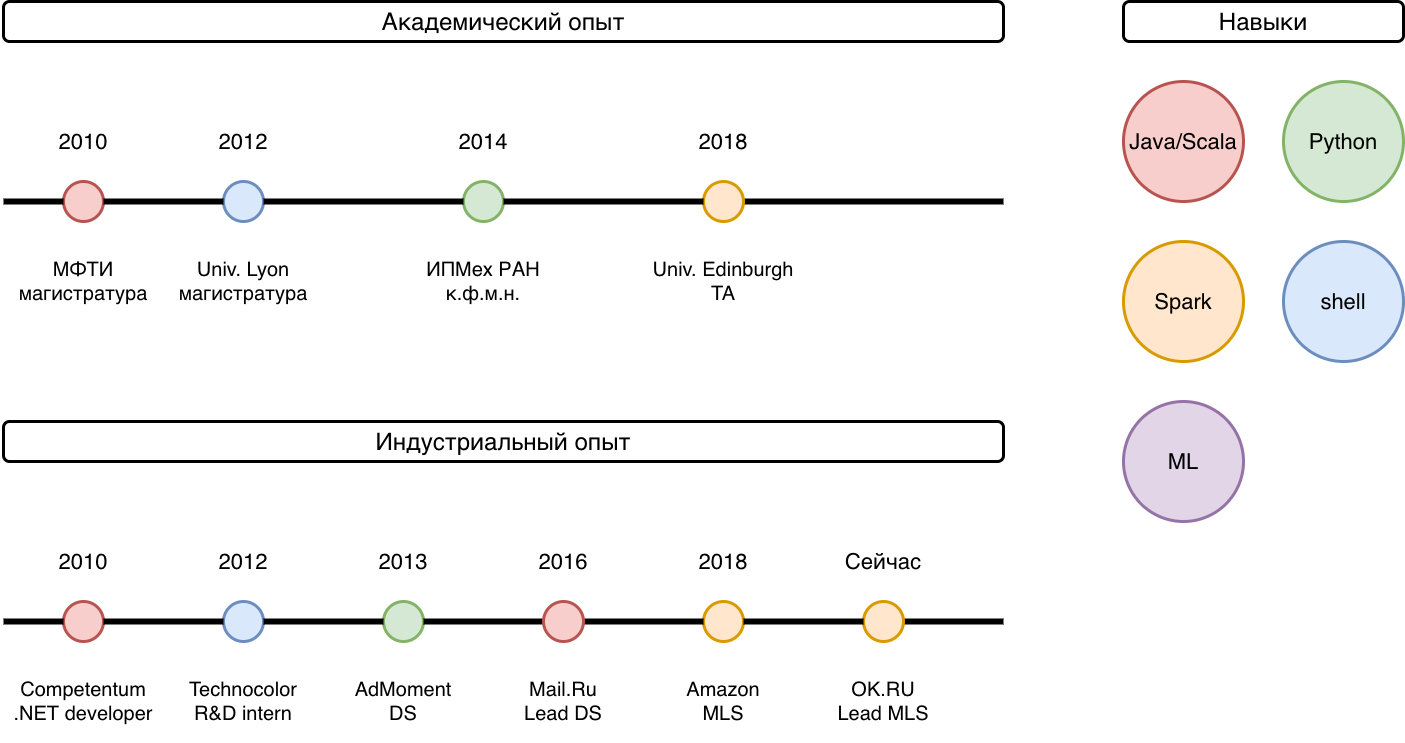
\includegraphics[scale=0.23]{images/about-me.png}
\end{center}

\end{frame}

\begin{frame}{Telegram}

\begin{itemize}
\item Вопросы вне занятия можно задать в личных сообщениях и чате группы (лучше)
\item Тегайте меня, чтобы я не пропустил ваш комментарий в общем потоке сообщений
\item Если ответа не последовало в течении 24 часов, то я, вероятно, не увидел ваше сообщение. Не стесняйтесь его продублировать
\end{itemize}

\end{frame}

\begin{frame}{Как задать вопрос}

\begin{itemize}
\item Голосом
\item В специально выделенное для этого время
\item Перед тем как спросить будет хорошим тоном поставить несколько знаков вопроса
\begin{tcolorbox}[colback=gray!5,colframe=gray!80,title=]
20:23 Саша: ???? \\
20:23 Преподаватель: Ждём вопроса от Саши \\
20:24 Саша: Какая метрика хорошо работает в задаче рекомендаций?
\end{tcolorbox}
\end{itemize}

\end{frame}

\begin{frame}{Если что-то пошло не так}

\begin{itemize}
\item Пропал голос
\item Исчезло изображение
\item Плохо слышно
\item Любые проблемы другого характера
\end{itemize}
\vfill
{\bf Сразу пишем в чат} много минусов и не ждем других участников. Если вы увидели, что в чате кто-то написал много минусов, а у вас всё хорошо, то поставьте несколько плюсов:
\vfill
\begin{tcolorbox}[colback=gray!5,colframe=gray!80,title=]
20:24 Петя: - - - - - - -  \\
20:25 Саша: ++++ \\
20:25 Ольга: +++++++
\end{tcolorbox}

\end{frame}

\begin{frame}{Программа модуля}
\begin{tabular}{ l | l | c | c }
{\bf Дата} & {\bf Тема} & {\bf Семинар} & {\bf Домашка} \\
\hline
2021-09-30 & Рекомендательные сервисы в продакшене & \checked &  \\
2021-10-07 & Метрики и базовые подходы & \checked &  \\ 
2021-09-14 & Классические алгоритмы & \checked & \checked  \\
2021-09-21 & Нейросетевые рекомендеры & \checked &  \\
2021-09-28 & Нерешенные проблемы и новые направления & \checked & 
\end{tabular}
\end{frame}

\section{Зачем нужны рекомендательные сервисы}

\begin{frame}{}

\vfill
\begin{tcolorbox}[colback=info!5,colframe=info!80,title=]
{\bf Recommender Systems} (RS) are software tools and techniques providing suggestions for {\bf items} to be of use to a {\bf user} \cite{RSHB}.
\end{tcolorbox}
\vfill
\begin{center}
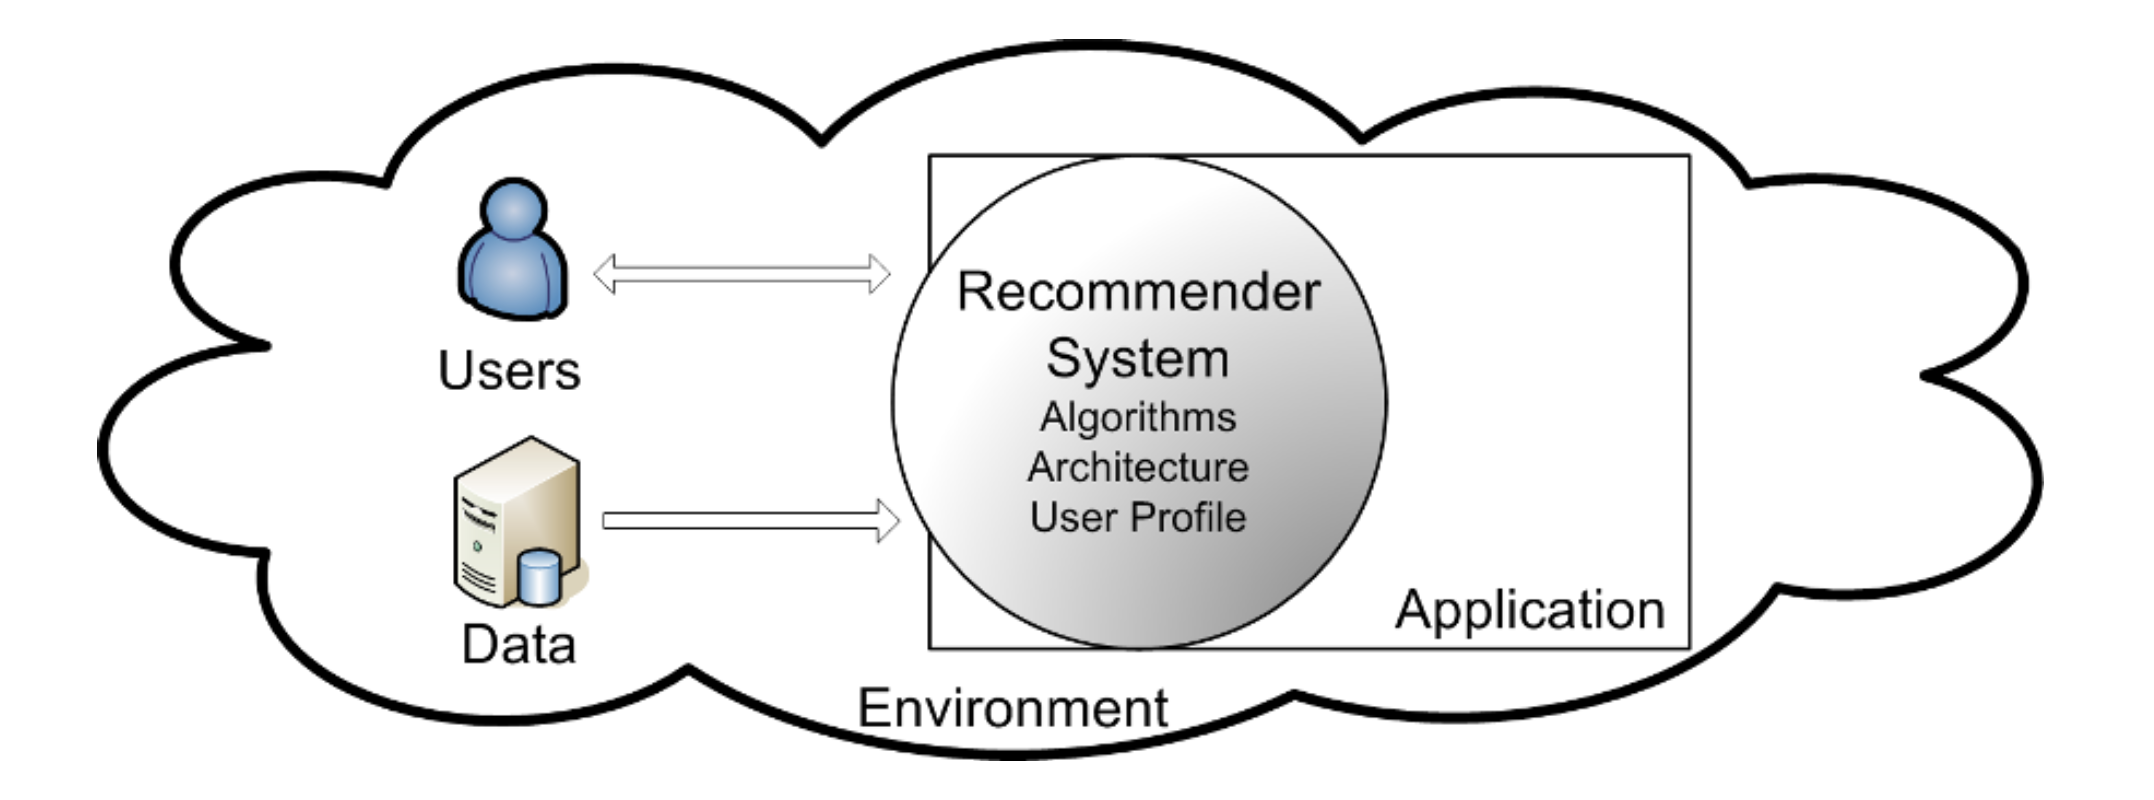
\includegraphics[scale=0.3]{images/overall.png}
\end{center}

\end{frame}

\begin{frame}{Зачем RS бизнесу}

\begin{itemize}[<+->]
\item Увеличить продажи
\item Продвигать более разнообразные товары
\item Улучшить пользовательский опыт
\item Добиться большей лояльности
\item Лучше понимать пользователей
\end{itemize}

\end{frame}

\begin{frame}{Зачем RS пользователям}

\begin{itemize}[<+->]
\item Найти лучший товар
\item Найти {\bf все} подходящие товары
\item Найти последовательность или набор товаров
\item Залипнуть
\item Найти рекомендер, которому можно доверять
\item Реализовать творческие потребности
\item Помочь другим сделать выбор
\end{itemize}

\end{frame}

\begin{frame}{Зачем RS инженерам}

\begin{itemize}
\item Делать высоконагруженный отказоустойчивый сервис
\item Анализировать большие данные
\item Окунуться в волшебный мир \sout{матана} машинного обучения
\item Объективно измерять результат своей работы 
\item Все это за зарплату
\end{itemize}

\end{frame}

\section{Архитектуры рекомендательных сервисов}

\begin{frame}{Обзор типичных компонентов RS / Mendeley (2016) \cite{MNDL}}
% Components
\begin{columns}
\begin{column}{0.6\textwidth}
   \begin{center}
		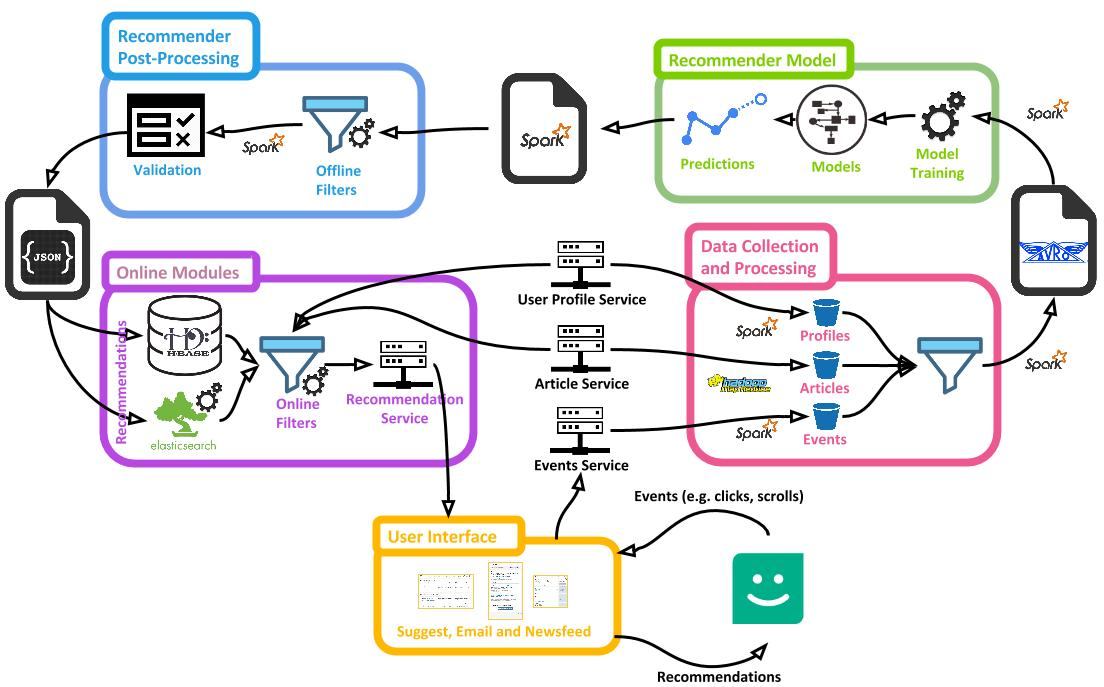
\includegraphics[scale=0.2]{images/mendeley.jpeg}
   \end{center}
\end{column}
\begin{column}{0.3\textwidth}
    \begin{tcolorbox}[colback=info!5,colframe=info!80,title=]
    Машинное обучение -- небольшая часть рекомендательного сервиса
    \end{tcolorbox}
\end{column}
\end{columns}

\end{frame}

\begin{frame}{Подходы к обработке данных / Netflix (2013) \cite{NFLX}}
% Online vs Nearline vs Offlie
\begin{columns}
\begin{column}{0.6\textwidth}
   \begin{center}
		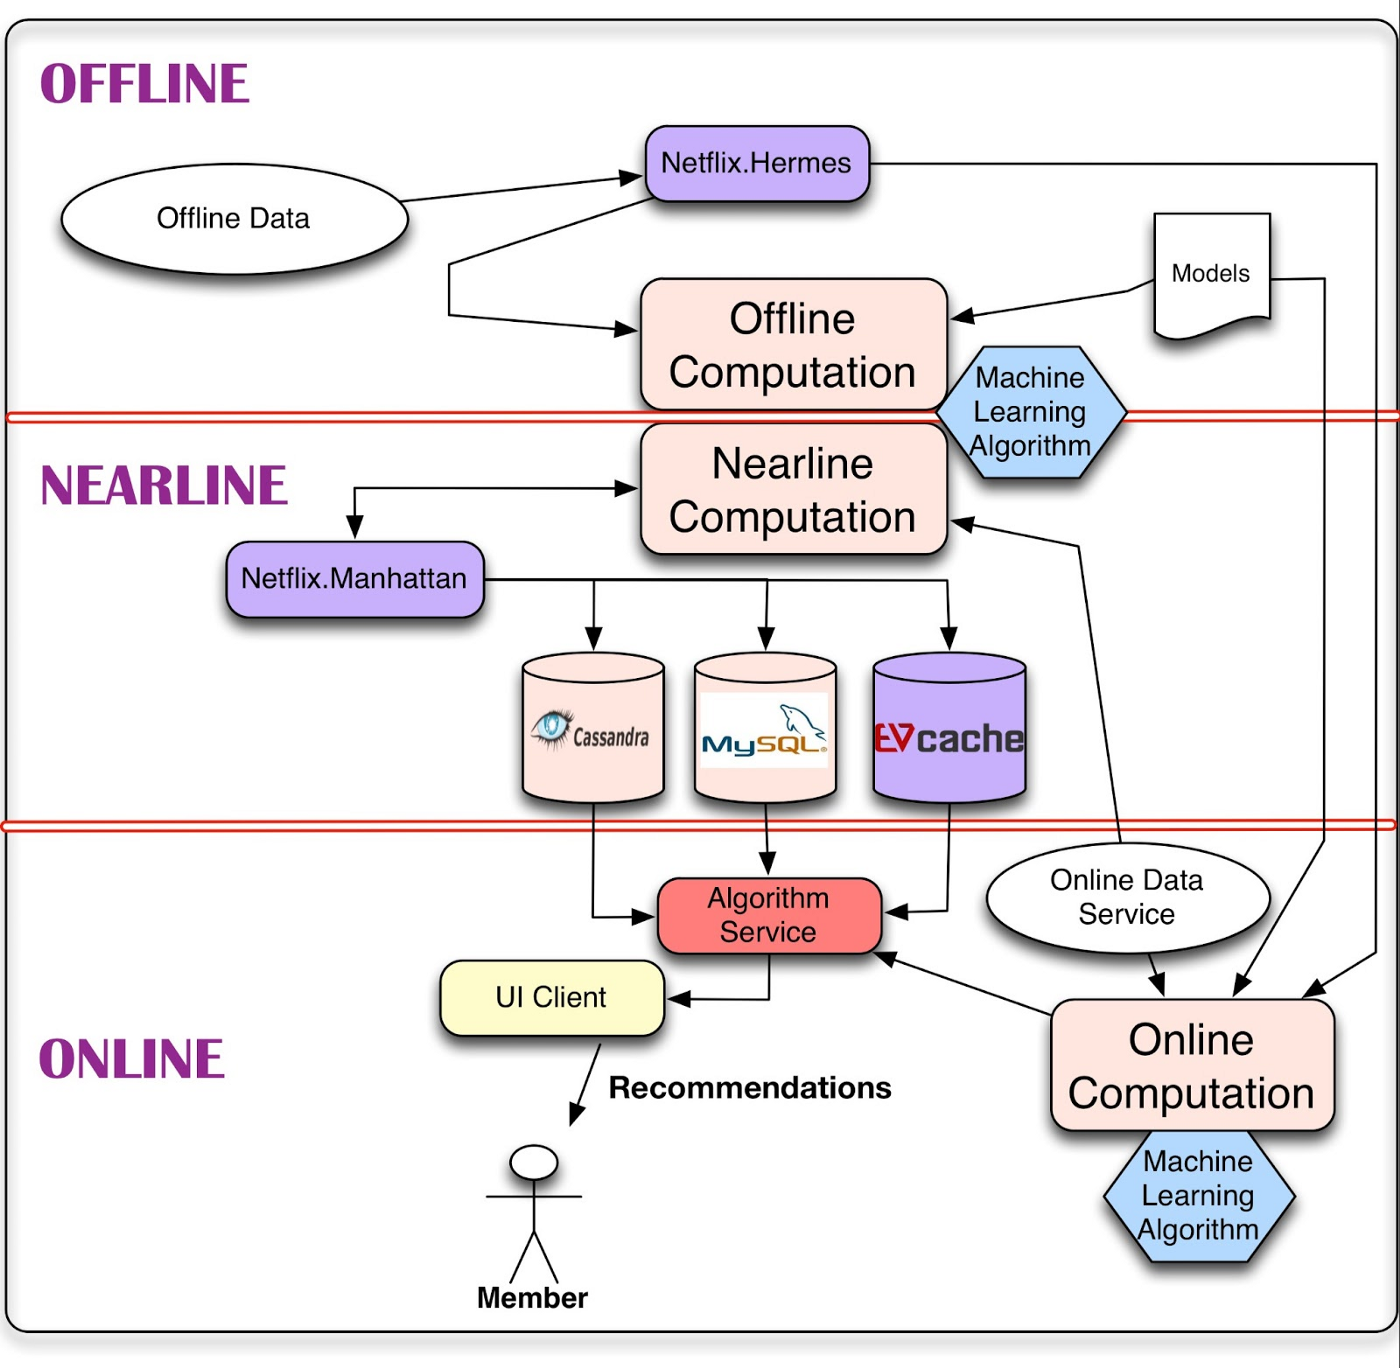
\includegraphics[scale=0.13]{images/netflix.png}
   \end{center}
\end{column}
\begin{column}{0.3\textwidth}
    \begin{tcolorbox}[colback=info!5,colframe=info!80,title=]
    Чем ближе вычисления к real-time, тем больше ограничений и компромиссов
    \end{tcolorbox}
\end{column}
\end{columns}

\end{frame}

\begin{frame}{Двухступенчатая архитектура / Youtube (2016) \cite{YTBE}}
% Enormous action space, context
\begin{columns}
\begin{column}{0.6\textwidth}
   \begin{center}
		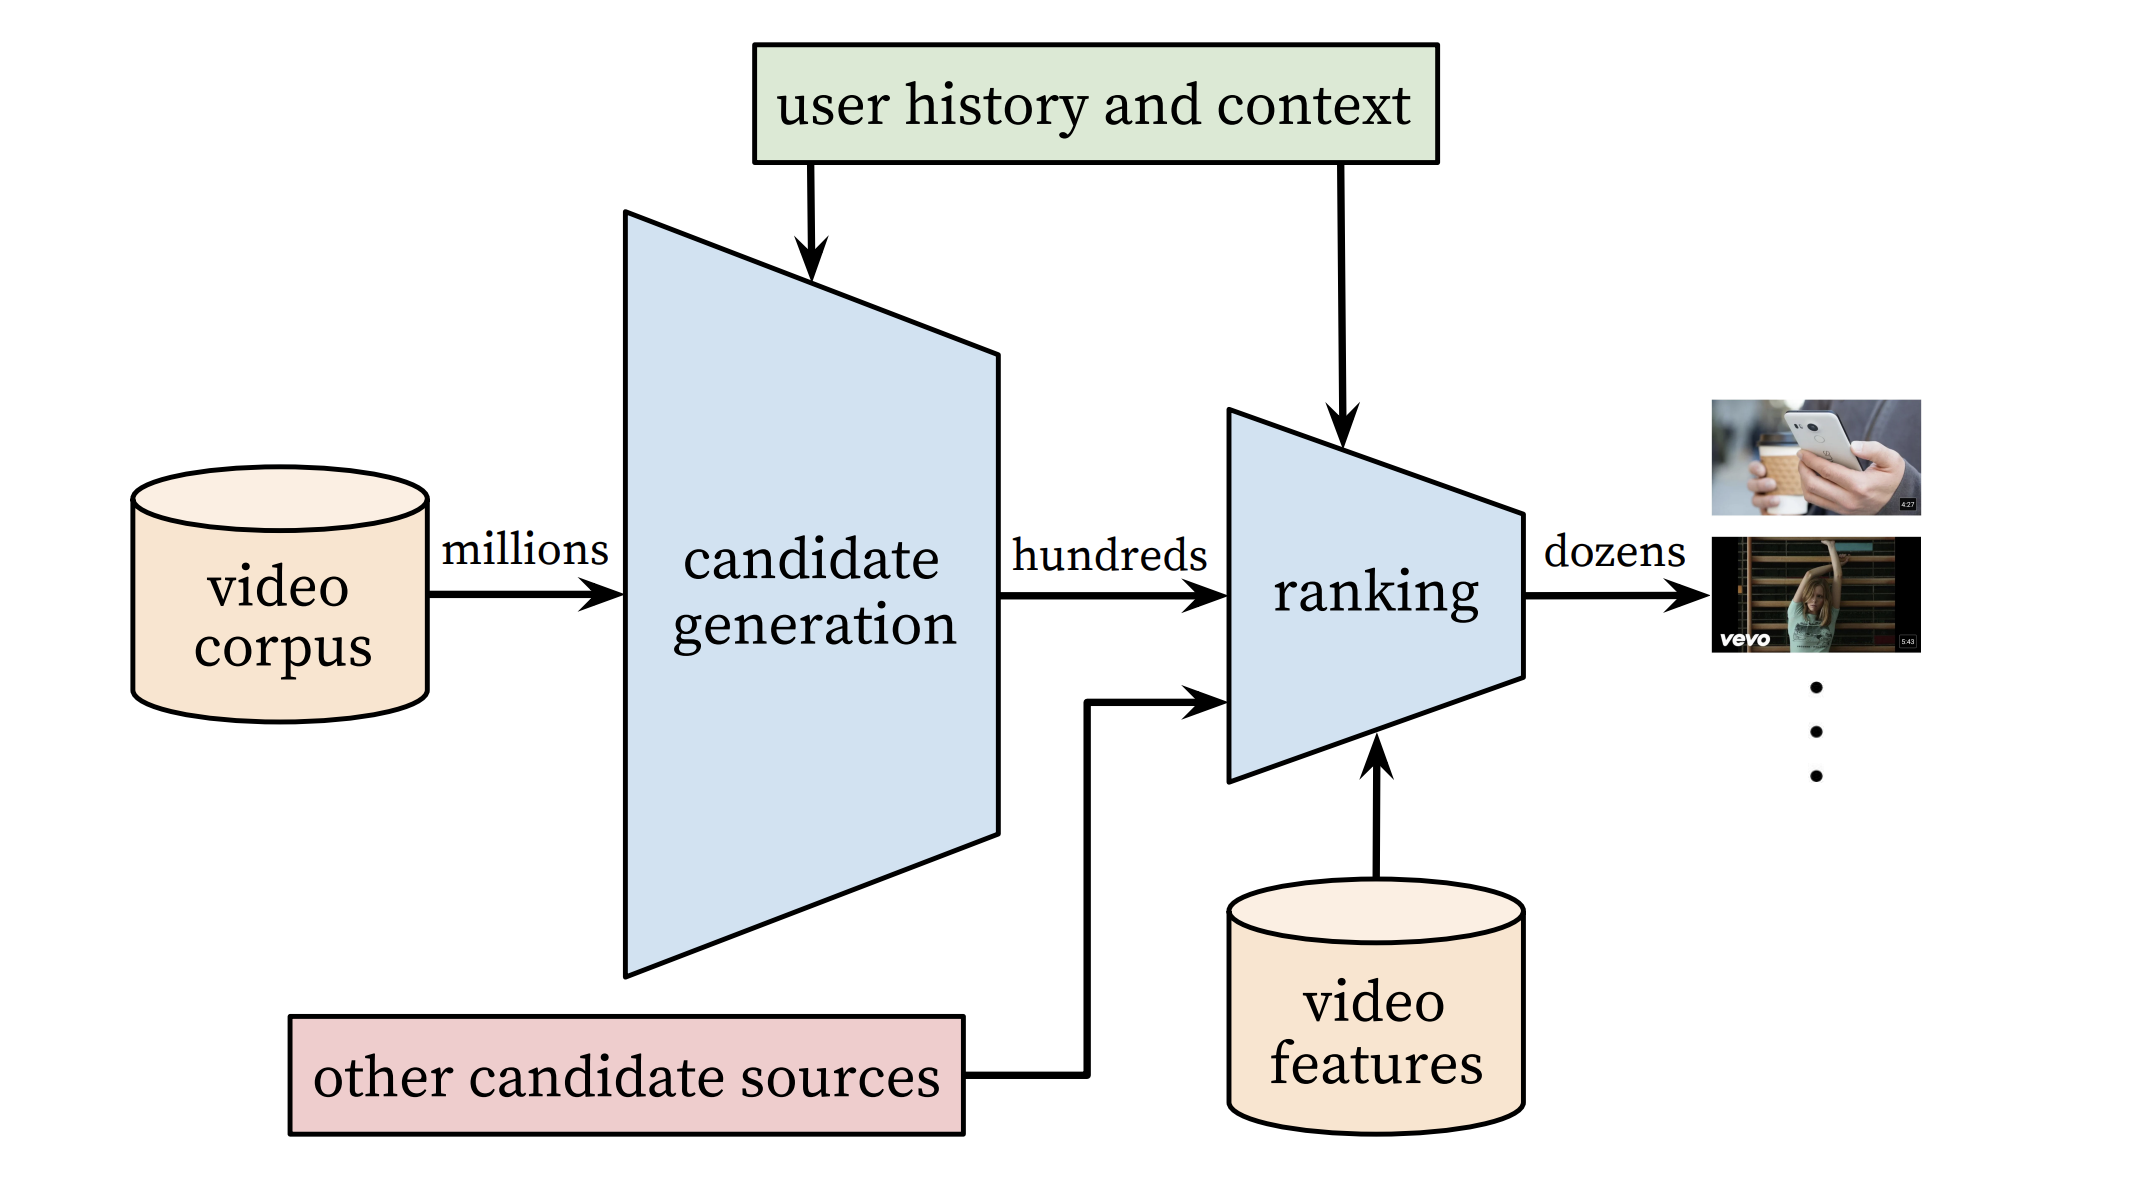
\includegraphics[scale=0.25]{images/youtube.png}
   \end{center}
\end{column}
\begin{column}{0.3\textwidth}
    \begin{tcolorbox}[colback=info!5,colframe=info!80,title=]
    Айтемов так много, что учесть {\bf полный контекст} не может даже Google
    \end{tcolorbox}
\end{column}
\end{columns}

\end{frame}

\begin{frame}{Загадка}

Что общего между
\begin{itemize}
\item населением городов
\item количеством друзей у пользователей в социальной сети
\item размерами лесных массивов
\item количеством прослушиваний песен в Spotify
\end{itemize}

\end{frame}

\begin{frame}{Power law}

\[
p(x) = \frac{C} {x^{\alpha}}, \quad x > x_{min}
\]

\begin{center}

\includegraphics[scale=0.25]{images/longtail.png}

Правило 80/20
\end{center}

\end{frame}

\begin{frame}{Холодный старт и длинный хвост / Spotify (2016) \cite{SPTF}}
% Long tail, coldstart
\begin{columns}
\begin{column}{0.6\textwidth}
   \begin{center}
		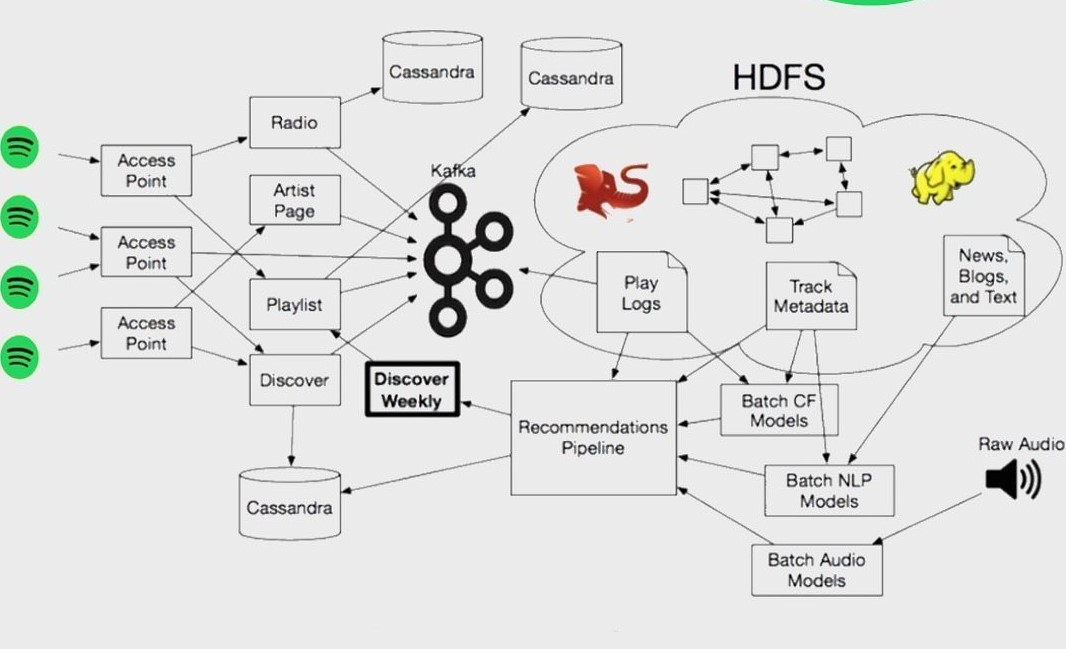
\includegraphics[scale=0.31]{images/spotify.jpeg}
   \end{center}
\end{column}
\begin{column}{0.3\textwidth}
    \begin{tcolorbox}[colback=info!5,colframe=info!80,title=]
    Холодные айтемы и пользователи будут всегда: думаем, что с ними делать
    \end{tcolorbox}
\end{column}
\end{columns}

\end{frame}

\begin{frame}{Работа с контентом / TikTok (2020) \cite{TIK}}
% Intangible objectives, content, exploration/authors!
\begin{columns}
\begin{column}{0.6\textwidth}
   \begin{center}
		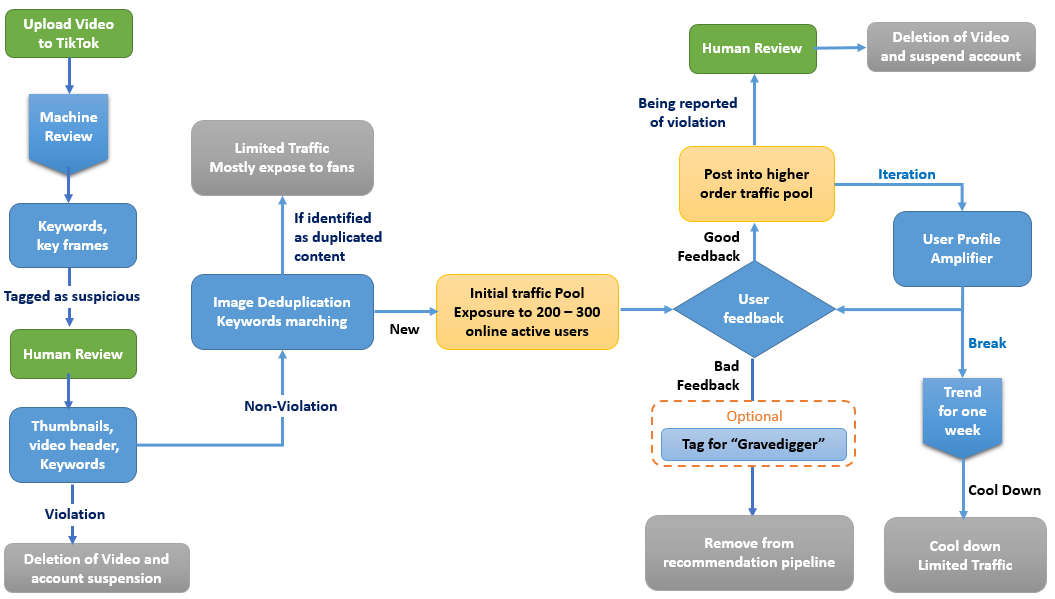
\includegraphics[scale=0.24]{images/tiktok.png}
   \end{center}
\end{column}
\begin{column}{0.3\textwidth}
    \begin{tcolorbox}[colback=info!5,colframe=info!80,title=]
    Потребности людей нельзя упаковать в удобную метрику: вокруг МЛ нужен пре- и пост-процессинг
    \end{tcolorbox}
\end{column}
\end{columns}

\end{frame}

\begin{frame}{Как в действительности выглядит архитектура RS}

\begin{center}
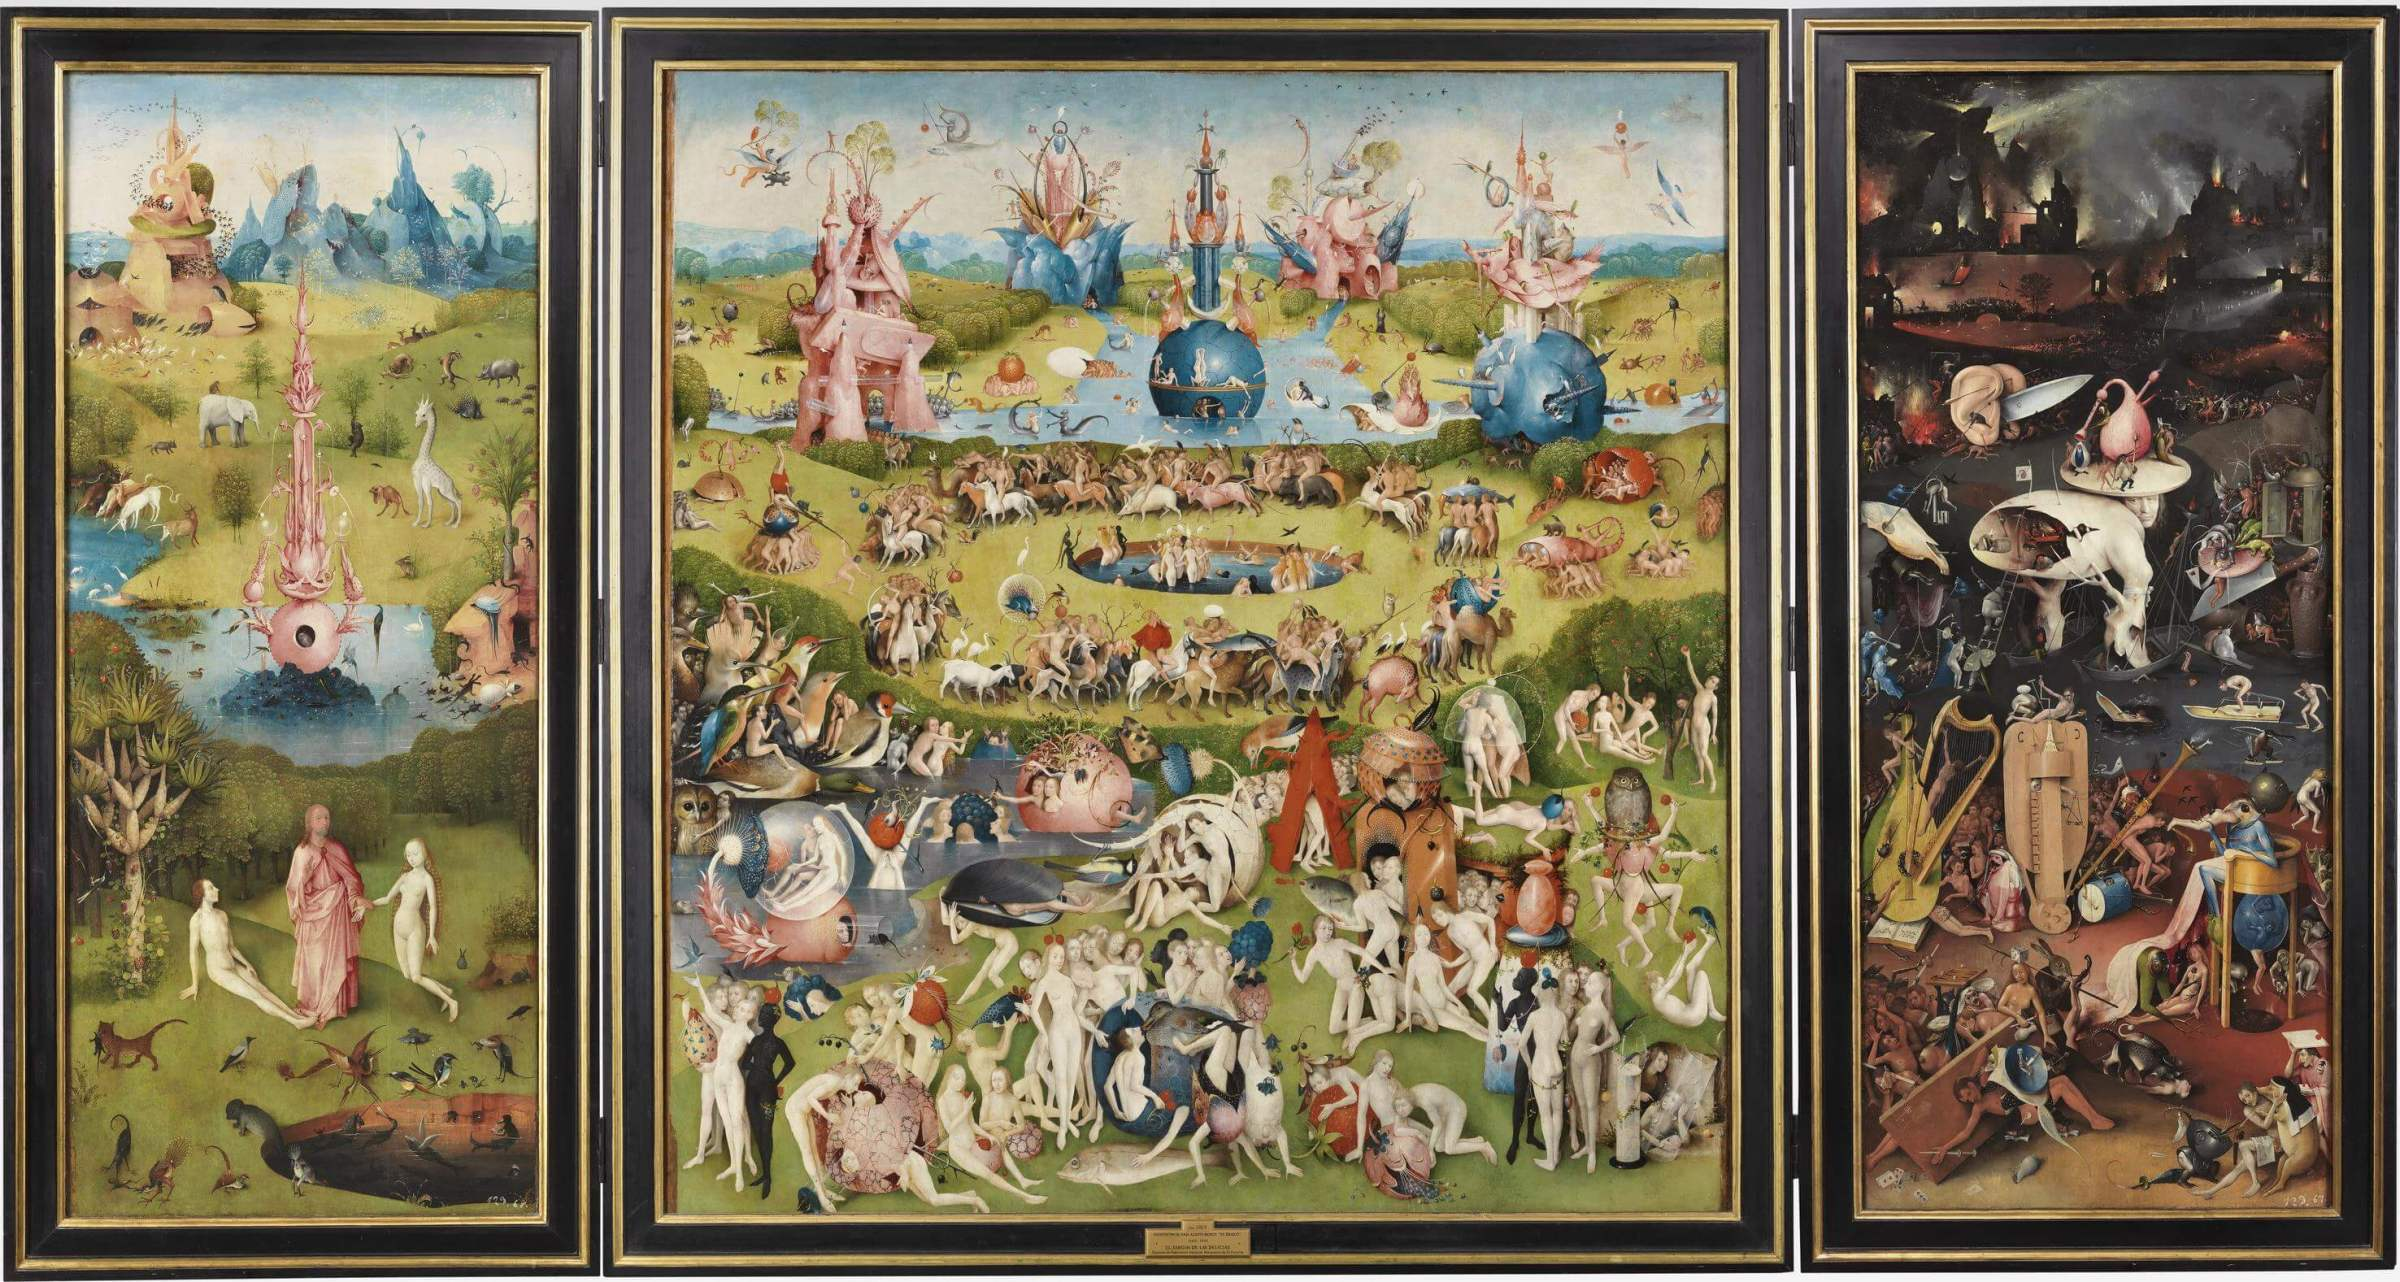
\includegraphics[scale=0.15]{images/bosch.jpeg}
\end{center}

\end{frame}

\section{Метрики и эксперименты}

\begin{frame}{}

Хотим принимать решения на основе данных $\rightarrow$ 

\qquad Начинаем собирать метрики $\rightarrow$ 

\qquad \qquad Разрабатываем инструменты для анализа метрик

\end{frame}

\begin{frame}{}

\begin{tcolorbox}[colback=info!5,colframe=info!80,title=Задача]
Какой эффект на распределение целевой метрики окажет выбранное воздействие $T$?
\end{tcolorbox}

\vfill

\begin{tcolorbox}[colback=warn!5,colframe=warn!80,title=Фундаментальная Проблема Causal Inference]
Для конкретного объекта невозможно вычислить causal effect напрямую, потому что нельзя пронаблюдать значение целевой переменной при более чем одном значении $T$\footnote{Без дополнительных предположений эту проблему не решить \cite{GELMAN}}
\end{tcolorbox}

\end{frame}

\begin{frame}{Фреймворк Potential Outcomes}

Воздействие на $i$ пользователя:
\[
T_i = \begin{cases}
0, \quad \text{если показываем сontrol} \\
1, \quad \text{если показываем treatment}
\end{cases}
\]

Соответствующие потенциальные исходы:
\[
y_i^0 \text{ и } y_i^1
\]

Требуется оценить:
\begin{tcolorbox}[colback=info!5,colframe=info!80,title=Average Treatment Effect,center,width=6cm,center title]
\[
ATE = E \left[ y_i^1 - y_i^0 \right]
\]
\end{tcolorbox}

\end{frame}

\begin{frame}{Randomized Controlled Experiment}

\begin{tcolorbox}[colback=info!5,colframe=info!80,title=Схема эксперимента]
Все доступные пользователи независимо друг от друга случайным образом распределяются в control либо treatment с одинаковой вероятностью
\end{tcolorbox}

\end{frame}

\begin{frame}{\phantom{Предположения RCE}}

\begin{tcolorbox}[colback=warn!5,colframe=warn!80,title=Предположение 1: ]
Можно оценить значение некоторой характеристики для всей популяции, имея выборку из этой популяции.
\end{tcolorbox}

\vfill

\begin{tcolorbox}[colback=warn!5,colframe=warn!80,title=Предположение 2: Stable Unit Treatment Value Assumption]
Потенциальные исходы для каждого пользователя зависят только от свойств этого пользователя, но не свойств и исходов других пользователей.
\end{tcolorbox}

\end{frame}

\begin{frame}{Оцениваем ATE в RCE}

\[
ATE = E[y_i^1 - y_i^0] = E[y_i^1] - E[y_i^0] \sim \text{avg}_{i \in T}(y_i^1) - \text{avg}_{i \in C}(y_i^0) = \bar y_1 - \bar y_0
\]

\begin{itemize}
\item нужно оценить две характеристики -- $E[y_i^0]$ и $E[y_i^1]$, поэтому используем выборки $C$ и $T$
\item проще всего сделать оценку, если выборка несмещенная
\item чем больше данных, тем точнее оценка
\end{itemize}

\end{frame}

\begin{frame}{Доверительный интервал на ATE}

Доверительный интервал $(L, U)$ с уровнем доверия $\alpha$:
\[
P(L < \theta < U) = 1 - \alpha
\]

Формула Уэлча:
\[
\bar y_1 - \bar y_0 \pm t_{\alpha/2,r} \sqrt{\frac{s_1^2}{n_1} + \frac{s_0^2}{n_0}}, \quad
r = \frac{ \left( \frac{s_1^2}{n_1} + \frac{s_0^2}{n_0} \right)^2 }{ \frac{s_1^4}{n_1^2 (n_1 - 1)} + \frac{s_0^4}{n_0^2 (n_0 - 1)} }
\]
Где:
\begin{itemize}
\item $n_1$ и $n_0$ -- количество пользователей в treatment и control
\item $s_1^2$ и $s_0^2$ -- оценки дисперсии метрики в treatment и control
\item $t_{\alpha/2,r}$ -- табличное значение для $r$ степеней свободы
\end{itemize}

\end{frame}

\begin{frame}{На практике}

\begin{itemize}
\item Метрики распределены по-разному: нужно подбирать подходящие тесты
\item Используются методы снижения дисперсии оценок (cuped, diff-in-diff)
\item Собираются тысячи метрик: часто для интерпретации нужны специалисты
\end{itemize}

\vfill

\begin{tcolorbox}[colback=info!5,colframe=info!80]
Если вы попали в компанию, в которой есть культура принятия решений на основе данных -- сохраняйте ее всеми силами. Если нет -- пропагандируйте.
\end{tcolorbox}

\end{frame}

\section{Итоги}

\begin{frame}
\begin{tcolorbox}[colback=info!5,colframe=info!80]
Рекомендательные сервисы улучшают жизнь бизнесу и пользователям. Жизнь инженеров они делают очень интересной.
\end{tcolorbox}
\vfill
\begin{tcolorbox}[colback=info!5,colframe=info!80]
В основе рекомендательных сервисов лежит машинное обучение. При проектировании  нужно учитывать множество дополнительных факторов, например требования к скорости обработки данных, эффект длинного хвоста и возможность холодного старта.
\end{tcolorbox}
\vfill
\begin{tcolorbox}[colback=info!5,colframe=info!80]
A/B эксперимент -- надежный способ оценки эффекта от изменений в сервисе.
\end{tcolorbox}

\end{frame}

\begin{frame}[allowframebreaks]{Литература}

\bibliographystyle{amsalpha}
\bibliography{references.bib}

\end{frame}

\end{document}
